%This template was prepared by Dorothea F. Brosius of the 
%Institute for Electronics and Applied Physics, University of Maryland, College Park, MD
%The template was last updated in March 2013
%Thesis Main Page used with thesis.sty based on the
%University of Maryland Electronic Thesis and Dissertation (ETD) Style Guide

\documentclass[12pt]{thesis}  %12pt is larger than 11pt
%\usepackage[pctex32]{graphics}
\usepackage{titlesec}
   \titleformat{\chapter}
      {\normalfont\large}{Chapter \thechapter:}{1em}{}
 
\usepackage{graphicx}
\usepackage{cite}
\usepackage{lscape}
\usepackage{indentfirst}
\usepackage{latexsym}
\usepackage{multirow}
\usepackage{tabls}
\usepackage{wrapfig}
\usepackage{slashbox}
\usepackage{longtable}
\usepackage{supertabular}
\usepackage{subeqn}
\usepackage{subfigure}

\newcommand{\tbsp}{\rule{0pt}{18pt}} %used to get a vertical distance after \hline
\renewcommand{\baselinestretch}{2}
\setlength{\textwidth}{5.9in}
\setlength{\textheight}{9in}
\setlength{\topmargin}{-.50in}
%\setlength{\topmargin}{0in}    %use this setting if the printer makes the the top margin 1/2 inch instead of 1 inch
\setlength{\oddsidemargin}{.55in}
\setlength{\parindent}{.4in}
\pagestyle{empty}

\begin{document}

%Abstract Page 

\hbox{\ }

\renewcommand{\baselinestretch}{1}
\small \normalsize

\begin{center}
\large{{ABSTRACT}} 

\vspace{3em} 

\end{center}
\hspace{-.15in}
\begin{tabular}{ll}
Title of dissertation:    & {\large A Search for the Neutrinoless Double Beta Decay}\\
&                           {\large of Xenon-136 with Improved} \\
&                           {\large Sensitivity from Waveform Denoising} \\
\ \\
&                          {\large  Clayton G. Davis, Doctor of Philosophy, 2014} \\
\ \\
Dissertation directed by: & {\large  Professor Carter Hall} \\
&  				{\large	 Department of Physics } \\
\end{tabular}

\vspace{3em}

\renewcommand{\baselinestretch}{2}
\large \normalsize

\singlespace{
The EXO-200 detector is designed to search for a theorized decay process of xenon-136 called neutrinoless double-beta ($\beta\beta 0\nu$) decay.  $\beta\beta 0\nu$ decay, if it occurs, would have important consequences for our understanding of the neutrino sector of the standard model.  It would demonstrate the type of the neutrino mass term; set the mass scale of the neutrino sector; and demonstrate the first direct observation of lepton number non-conservation.  The $\beta\beta 0\nu$ decay produces a monoenergetic peak, so one important approach to reducing backgrounds for this search is by improving the energy resolution of the detector.

The present work describes a new analysis technique which improves resolution in the scintillation channel by a combination of waveform denoising and weighting of waveform components based on their expected signal-to-noise ratio; the overall resolution of the detector is improved by better than $20\%$.  Application of this method results in a halflife limit on $\beta\beta 0\nu$ decay in xenon-136 of $T_{1/2} > 1.1 \cdot 10^{25}$ years at $90\%$ confidence.  Further improvements which could impact the energy resolution of EXO-200 are also described, and implications for the planned nEXO experiment are considered.
}
 %(must be first, required, non-numbered)
%Titlepage

\thispagestyle{empty}
\hbox{\ }
\vspace{1in}
\renewcommand{\baselinestretch}{1}
\small\normalsize
\begin{center}

\large{{SIGNAL DENOISING FOR EXO-200 AND AN IMPROVED LIMIT ON NEUTRINOLESS DOUBLE-BETA DECAY}}\\
\ \\
\ \\
\large{by} \\
\ \\
\large{Clayton G. Davis}%Your full name as it appears in University records.
\ \\
\ \\
\ \\
\ \\
\normalsize
Dissertation submitted to the Faculty of the Graduate School of the \\
University of Maryland, College Park in partial fulfillment \\
of the requirements for the degree of \\
Doctor of Philosophy \\
2014
\end{center}

\vspace{7.5em}

\noindent Advisory Committee: \\
Professor Carter Hall, Chair/Advisor \\
Professor Radu Balan \\
Professor Betsy Beise \\
Professor Rabindra Mohapatra \\
Professor Peter Shawhan
 %(must follow Abstract, required, non-numbered)
%Copyright

\thispagestyle{empty}
\hbox{\ }

\vfill
\renewcommand{\baselinestretch}{1}
\small\normalsize

\vspace{-.65in}

\begin{center}
\large{\copyright \hbox{ }Copyright by\\
Clayton Davis  %Type your name as it appears in University records
\\
2014}
\end{center}

\vfill
 %(highly recommended, non-numbered)

%Pages from this point start at lower-case Roman number ii)
\pagestyle{plain}
\pagenumbering{roman}
\setcounter{page}{2}

%Preface

\renewcommand{\baselinestretch}{2}
\small\normalsize
\hbox{\ }
 
\vspace{-.65in}

\begin{center}
\large{Preface} 
\end{center} 


If needed.
  %(if present, start at lower-case Roman number ii)
%Foreword

\renewcommand{\baselinestretch}{2}
\small\normalsize
\hbox{\ }
 
\vspace{-.65in}

\begin{center}
\large{Foreword} 
\end{center} 

If needed.
 %(if present, lower-case Roman)
%Dedication

\renewcommand{\baselinestretch}{2}
\small\normalsize
\hbox{\ }
 
\vspace{-.65in}

\begin{center}
\large{Dedication}
\end{center} 

If needed.
 %(if present, lower-case Roman)
%Acknowledgments

\renewcommand{\baselinestretch}{2}
\small\normalsize
\hbox{\ }
 
\vspace{-.65in}

\begin{center}
\large{Acknowledgments} 
\end{center} 

\vspace{1ex}

Without the help of my colleagues, advisor, friends, family, and my wife, this thesis and the work it embodies would never have happened.  I would like to give thanks to the EXO-200 collaboration, which has provided a supportive and stimulating environment for my work and learning over the past four years.

Particular thanks must go to: David Auty, Phil Barbeau, Giorgio Gratta, Steve Herrin, Sam Homiller, Mike Jewell, Tessa Johnson, Tony Johnson, Caio Licciardi, Mike Marino, Dave Moore, Russell Neilson, Igor Ostrovskiy, J.J. Russell, Kevin O'Sullivan, Tony Waite, Josiah Walton, Liangjian Wen, Liang Yang, and of course my advisor Carter Hall.  I can honestly say that each one of you directly made the following work possible with your contribution of insight, data, plots, and analysis.  Denoising has been a tremendously collaborative effort, and I am grateful that my last project with this group has provided the chance to work with all of you so closely.
 %(if present, lower-case Roman)

\renewcommand{\baselinestretch}{1}
\small\normalsize
\tableofcontents %(required, lower-case Roman)
\newpage
%\listoftables %(if present, lower-case Roman)
%\newpage
\listoffigures %(if present, lower-case Roman)
\newpage
% LIST OF ABBREVIATIONS
\addcontentsline{toc}{chapter}{List of Abbreviations}
%List of Abbreviations

\renewcommand{\baselinestretch}{1}
\small\normalsize
\hbox{\ }

\vspace{-4em}

\begin{center}
\large{List of Abbreviations}
\end{center} 

\vspace{3pt}

\begin{tabular}{ll}
EXO & Enriched Xenon Observatory \\
APD & Avalanche Photo-diode \\
\end{tabular}


\newpage
\setlength{\parskip}{0em}
\renewcommand{\baselinestretch}{2}
\small\normalsize

%Pages from this point start at Arabic numeral 1
\setcounter{page}{1}
\pagenumbering{arabic}
%Chapter 1

\renewcommand{\thechapter}{1}

\chapter{Introduction}

\section{Source of Nonlinearity in an Optical Fiber}

	The response of any dielectric to light becomes nonlinear
for intense electromagnetic fields.  Standard optical fibers are made of
fused silica which is a dielectric. The total polarization $\bf{P}$
is nonlinear in the electric field $\bf{E}$ and is given by [1-5] -
%\cite{Agrawal1,Bloembergen,Shen,Butcher,Boyd} -
%1.1
\begin{equation}
{\bf P} = \epsilon_{0} \left( \chi^{(1)} : {\bf E} + \chi^{(2)} 
: {\bf EE} + \chi^{(3)} : {\bf EEE} + \ldots \right),
\end{equation}
where $\epsilon_0$ is the permittivity of free-space, and
$\chi^{(j)}$ 
is the ${\it j}$-th order susceptibility of the dielectric. The linear
susceptibility $\chi^{(1)}$ represents the dominant contribution to
$\bf{P}$ and its effects are included through the refractive index
n($\omega$) and the attenuation coefficient $\alpha(\omega)$. $\chi^{(2)}$
is responsible for nonlinear effects such as sum-frequency generation and
second harmonic generation \cite{Agrawal1, Shen}. Fused silica does not
manifest these effects as it is centro-symmetric \cite{Newell}. Hence, the dominant nonlinear
contribution to ${\bf P}$ is due to $\chi^{(3)}$ which results in effects
such as third harmonic generation, four-wave-mixing,  self- and
cross-phase modulation. The cubic nonlinearity results in an intensity
dependent refractive index

\begin{verbatim}
122	23333
1114	14444
\end{verbatim}

%1.2
\begin{equation}
\tilde{n}(\omega,|E|^2) = n(\omega)+n_2|E|^2 ,
\end{equation}
where n($\omega$) is the linear part given by the Sellmier
equation which
takes into account the resonance frequencies ($\omega_j$) of fused
silica \cite{Agrawal1,Marcuse},
%1.3
\begin{equation}
n^2(\omega) = 1 + \sum_{j=1}^m {B_j\omega^2_j \over \omega^2_j - \omega^2}
\end{equation}
and n$_2$ is given by
%1.4
\begin{equation}
n_2 = {3 \over 8n}Re(\chi_{xxxx}^3)
\end{equation}
for an optical wave assumed to be linearly polarized along one of the 
axes of a polarization maintaining fiber. The tensorial nature of $\chi^{(3)}$ needs to be
considered for the case in which the light is not polarized along one of
the fiber axes.\footnote{This is my footnote.  I started playing the piano when I was eight years old.  This is my footnote.  I started playing the piano when I was eight years old.  This is my footnote.  I started playing the piano when I was eight years old.  This is my footnote.  I started playing the piano when I was eight years old.}

The experimentally measured value of $n_{2}$ for fused silica ranges from $2.2 - 3.4 \times
10^{-20}$\,m$^2$/W, which is small compared to most other nonlinear media by
at least 2 orders of magnitude \cite{Agrawal1}. Despite this, nonlinear effects are
easily observed for silica fibers for relatively low input power levels due
to the fact that the effective fiber core areas are small and the fiber losses are low. Single mode fibers (those which propagate a single transverse mode of light for a given wavelength) have effective fiber core diameters of the order of 5$\mu$m thus causing the light intensities within the fiber to be large despite the smallness of the input power. The low loss in the fiber ($<$10 dB/km) allows one to use long fibers to observe nonlinear phenomena.

\section{Physics of Pulse Propagation}

Mathematically speaking, in the classical limit, pulse propagation in an
optical fiber is governed by Maxwell's equations \cite{Agrawal2,Diament}, 
%1.5
\begin{eqnarray} 
\vec{\nabla}\times\vec{E} & = &- {\partial \vec{B} \over \partial t} \nonumber\\
\vec{\nabla}\times\vec{H} & = & \vec{J}+ {\partial \vec{D} \over \partial t}
\nonumber\\ 
\vec{\nabla}\cdot\vec{D} & = & \rho_{f} \nonumber\\
\vec{\nabla}\cdot\vec{B} & = & 0 ,
\end{eqnarray}
where $\vec{E}$ and $\vec{H}$ are electric and magnetic field
vectors, and
$\vec{D}$ and $\vec{B}$ are electric and magnetic flux densities, 
respectively. $\vec{J}$ is the current density and $\rho_{f}$ is the free
charge density.

Under the following assumptions \cite{Agrawal2} -
\begin{enumerate}
\item[(a)]
there are no free charges ($\vec{J}=\rho_{f}=0$), a good approximation for an optical fiber, 
\item[(b)] the medium is non-magnetic ($\vec{M}=0$), which an optical fiber is,
\item[(c)] the wavelength of light propagated is away from any material
resonances (0.5 - 2 $\mu$m), the results described in this thesis lie in this wavelength range, i.e., the results presented in Chap.\ 2 and Chap.\ 3 lie in the 600-700\,nm regime and the results presented in Chap.\ 4 lie in the 800\,nm regime,
\item[(d)] the electric-dipole approximation is valid, due to which the second-order parametric processes such as three-wave-mixing and second harmonic generation can be neglected (in practice they do occur because of quadrupole and magnetic-dipole effects but with a very low efficiency),
\item[(e)] the medium only responds locally, which is a valid approximation for the projects considered herein,
\item[(f)] the nonlinear polarization $\vec{P}_{NL}$ can be taken as a
perturbation to the total induced polarization $\vec{P}$, which is justified as the nonlinear effects are relatively weak for the results presented in this thesis,
\item[(g)] only 3rd order nonlinear effects need to be taken into
account, which is valid up to 5th order in ${\bf E}$ since the 2nd and 4th order effects are absent due to the centrosymmetric nature of the disordered liquidlike state of fused silica,
\item[(h)] the imaginary part of the dielectric constant
$\epsilon(\omega)$ is small compared to the real part (low loss, which is a good approximation for the wavelength regimes and fiber lengths considered here),
\item[(i)] the wavelength of light is higher than the cutoff wavelength
of the fiber so that the single transverse mode condition is satisfied (or else there would be multimode propagation and nonuniform modal dispersion would have to be taken into account),
\item[(j)] the optical fiber is polarization maintaining and the light
pulse is traveling along one of the 2 principal axes of the fiber, a very good approximation for the results of Chap.\ 2, and Chap.\ 3, in the case of Chap.\ 4, this approximation is relaxed as the incident light travels along both axes of the fiber, thus requiring a set of two coupled NLSEs for simulation, one for each axis,
\item[(k)] the slowly varying envelope approximation is valid, i.e.,
$\Delta\omega/\omega_{0} \ll 1$ where $\Delta \omega$ is the spectral
width of the pulse spectrum which is centered at $\omega_{0}$, this approximation is valid for the studies considered in Chap.\ 2 and Chap.\ 4, in Chap.\ 3, the Raman Stokes wave is considered as a separate slowly varying envelope from the pump wave, as the two taken together would not satisfy this condition,
\item[(l)] the nonlinear response of the medium is instantaneous, an
approximation valid for pulse widths greater than $\sim$70\,fs, which amounts to neglecting the contribution of molecular vibrations to $\chi^{(3)}$ (the Raman effect), which have been included in the study presented in Chap.\ 4 since the pulse width was $\sim$ 140\,fs.
\end{enumerate}
The propagation of the slowly varying envelope A(z,t) of a light
pulse
along an optical fiber is governed by the nonlinear partial
differential equation \cite{Agrawal2} -
%1.6
\begin{equation}
{\partial A \over \partial z} + \beta_{1} {\partial A \over \partial t} + {i \beta_{2} \over 2} {\partial^{2} A \over \partial t^{2}} = i \gamma |A|^{2}A,
\end{equation}
where $v_{g}=1/\beta_{1}$ is the group velocity of the pulse,
$\beta_{2}$
is the group velocity dispersion coefficient, %$\alpha$ is the fiber loss,
and $\gamma$ is the nonlinearity coefficient given by
%1.7
\begin{equation}
\gamma = {n_{2}\omega_{0} \over c A_{eff}} .
\end{equation}

Here $\omega_{0}$ is the central angular frequency of the pulse and
A$_{eff}$, the effective core area of the fiber.

Under transformation to  a frame of reference moving at the group
velocity of the pulse, the above equation takes the form of the so-called
`nonlinear Schr\"odinger equation' (NLSE), i.e.,
%1.8
\begin{equation}
{\partial A \over \partial z} + {i\beta_2 \over 2} {\partial^2
A \over \partial \tau^2} = i \gamma |A|^2A ,
\end{equation}
where
%1.9
\begin{equation}
\tau = t - {z \over v_g}
\end{equation}
is time measured in a frame of reference moving at the group
velocity
v$_g$ of the pulse.

\section{Numerical Pulse Propagation}

The NLSE, like most nonlinear partial differential equations, is not
amenable to analytical solution except in certain special cases where the
inverse scattering transform can be used \cite{Zakharov}. Thus a
numerical approach is necessary for understanding the physics of phenomena
governed by the NLSE. The numerical methods available can be classified as
finite-difference techniques and pseudo-spectral techniques. Usually
pseudo-spectral methods are an order of magnitude faster, the most
popular method being the Split-Step Fourier Method (SSFM) \cite{Agrawal2,Hardin,
Fisher}. The speed of the SSFM can be partly attributed to the use
of the finite fast-Fourier transform (FFT) algorithm
\cite{Cooley}.For an algorithmic description of the SSFM the reader is
referred to Chap.\ 2, Sec.\ 2. Therein is also described an
unconditionally stable scheme for including linear multiplicative noise into
the SSFM without disturbing the conservative properties of the NLSE. In the
projects described in Chap.\ 3, simulations were carried out using a
combination of the SSFM and finite difference schemes. The SSFM is also used 
 to arrive at the simulated results described in Chap.\ 4.

\section{Experimental Pulse Diagnostics}

With the advent of frequency resolved optical gating
(FROG) \cite{Trebino,Kanejqe,Kaneoptlett}, it has become possible to not
only measure the optical spectrum and optical time trace of a light pulse
but to measure the full electric field envelope (intensity and phase) of the
light pulse. The two fields of nonlinear fiber optics and frequency resolved
optical gating (FROG) are yet to undergo cross pollination to their fullest
potential since the inception of FROG 10 years ago. This novel experimental
technique adds new dimensions to pulse measurement techniques, one of which
is the ability to measure how asymmetric a pulse is, i.e., measure its
skewness, kurtosis and all higher order moments. Asymmetric pulse
propagation is a subject of interest in Chap.\ 4, where a highly simplified
version of FROG \cite{OShealett} is used to measure pulse characteristics
before and after a fiber.

\section{Group Velocity Dispersion}

Group velocity dispersion \cite{Agrawal3} (GVD) involves the temporal broadening of a pulse as it propagates through an optical fiber. From the NLSE (Eq.\ 1.6) one can derive length scales relevant to linear dispersion (L$_{D}$=T$_{0}^{2}$/$\beta_{2}$) and nonlinearity (L$_{NL}$=1/$\gamma$P$_{0}$). Here T$_{0}$ is the pulse width and P$_{0}$ is the peak power of the pulse. The regime in which the effects of GVD dominate and the effects of nonlinearity are negligible is given by -
%1.10
\begin{equation}
{L_{D} \over L_{NL}}={\gamma P_{0} T_{0}^{2} \over |\beta_{2}|} \ll 1 .
\end{equation}

In this regime, optical pulses propagate as they undergo symmetric temporal broadening and linear chirping without any spectral broadening. The sign of the GVD parameter $\beta_{2}$ determines the sign of the induced chirp. If the input pulse is chirped, then it may undergo some initial pulse compression followed by temporal broadening. Unlike the second-order dispersion associated with GVD, third-order dispersion causes asymmetric temporal broadening with leading and trailing edges. It becomes important, when the operating wavelength is near the zero dispersion wavelength of the fiber (the wavelength at which $\beta_{2}$=0). GVD starts to limit optical fiber communication systems when consecutive pulses broaden so much that they start to overlap.   

\section{Self-Phase Modulation}

Self-phase modulation \cite{Agrawal4} (SPM) is a phenomenon that leads to spectral broadening and modulation of optical pulses. In the absence of GVD, SPM induced spectral broadening occurs without change in the temporal pulse shape. The spectral broadening occurs as a consequence of an intensity dependent phase-shift. The project described in Chap.\ 2 has the property that L$_{NL}$ $<$ L $\ll$ L$_D$, i.e., the nonlinear term representing SPM dominates. In the regime where both SPM and GVD are non-negligible (as in Chap.\ 4), phenomena qualitatively different from those described in this section and the previous section can occur. Both temporal and spectral broadening can occur simultaneously. In the regime of femtosecond pulse propagation (as in Chap.\ 4), GVD, third-order dispersion, intrapulse Raman scattering (discussed in Chap.\ 2) and higher order nonlinear effects have to be taken into account. If the input pulse is asymmetric, then SPM effects dominate over all other effects, as is observed in Chap.\ 3. In some cases SPM can lead to pulse compression, and in the anomalous dispersion regime ($\beta_2 < 0$), the balance between GVD and SPM can lead to soliton formation. 

\section{Four-wave-mixing}

Four-wave-mixing (FWM) \cite{Agrawal10} is a parametric process involving
the interaction
between four photons at different frequencies. Two different kinds of
four-wave-mixing processes are possible -
%1.11
\begin{eqnarray}
\omega_4 = \omega_1 + \omega_2 + \omega_3 \\
\omega_3 + \omega_4 = \omega_1 + \omega_2 .
\end{eqnarray}

The former process results in third harmonic generation for the special case
when $\omega_1 = \omega_2 = \omega_3$. Both processes require phase
matching to occur, in order to be efficient. For the latter case, with
the partial degeneracy of $\omega_1 = \omega_2$, it is relatively easy
to satisfy the phase matching condition of
%1.12
\begin{equation}
\Delta k = k_3 + k_4 - k_1 - k_2 = 0 .
\end{equation}

This process is of great interest to nonlinear dynamicists as the
evolution of the FWM process could constitute a route to chaos further
down-stream in the fiber. It is also of great interest to people working in
the field of optical communication systems, as it can cause cross-talk
between neighboring channels in a wavelength division multiplexing scheme
of communication.

\section{Cross-Phase Modulation}

Cross-phase modulation (XPM) \cite{Agrawal7} occurs in optical fibers when
two or more optical pulses having different central wavelengths propagate 
simultaneously inside a fiber, interacting through the fiber
nonlinearity which couples the two pulses nonlinearly.  The evolution of the
two pulses depends on the group velocity mismatch between them by virtue of 
their being centered at different wavelengths, although this is a linear
phenomenon. The group velocity mismatch also exists between light pulses
traveling along orthogonal polarization axes of a fiber, and centered around
identical wavelengths, since the slow axis and fast axis of the fiber have
different group velocities. In this case, too, the two polarizations interact
nonlinearly \cite{Agrawal6} through degenerate XPM (degenerate since the
central wavelengths are the same). In the case of degenerate XPM the 2nd order 
and higher dispersion parameters, and the nonlinear parameters (all of which
depend only on the wavelength), are also the same unlike in general XPM. The effects of XPM are more pronounced when one of the pulses (the pump) has much higher power than the other (the probe). Otherwise, the effects of self-phase modulation (SPM) tend to dominate.

\section{Stimulated Inelastic Scattering} 

Other nonlinear effects (apart from those due to the cubic $\chi^{(3)}$
nonlinearity) arise due to the interaction between the light
traveling in the fiber and the fiber medium. Interactions between
the light field and the vibrational levels of the fiber medium lead to
stimulated Brillouin scattering (SBS) and stimulated Raman
scattering (SRS). SRS and SBS were among the first nonlinear effects
studied in optical fibers \cite{Stolen,Ippen,Smith}.  In a simple quantum
mechanical picture \cite{Agrawal1} applicable to
both SRS and SBS, a photon of the incident field (called the pump) is
annihilated to create a photon at a lower frequency (belonging to the
Stoke's wave) and a phonon to conserve energy and momentum. SBS involves
an acoustic phonon whereas SRS involves an optical phonon, thus they have
qualitatively different dispersion relations. SBS has a much
lower threshold power and manifest itself through a backward propagating
wave in contrast to SRS which can involve both forward and backward
traveling waves. SBS has a maximum gain at a frequency 10\,GHz \cite{Agrawal9}
(down-shifted with respect to the pump) and
requires a very narrow bandwidth pump to manifest itself. SRS, in
contrast, has a maximum gain at a frequency 13\,THz \cite{Agrawal8} downshifted with
respect to the pump. For pulse-bandwidths larger than 13\,THz, the
phenomenon of Intrapulse Raman Scattering (IRS) manifests itself,
involving a self-frequency shift within the pulse from higher frequency
components to lower frequency components. Thus, SRS
becomes more important for shorter pulses (larger bandwidth) unlike SBS
which nearly ceases to occur for pulses shorter than 10\,ns. In both SRS
and SBS, the optical fiber plays an active role in the nonlinear process,
unlike the case of cross- and self-phase modulation, four-wave-mixing and
third harmonic generation, where the fiber plays a passive role by
mediating the interaction between several optical waves.

\section{Outline of Thesis}

In Chap.\ 2, we present the results of a computational study of the
influence of stochasticity on the dynamical evolution of multiple 
four-wave-mixing processes in a single mode optical fiber with spatially
and temporally $\delta$-correlated phase noise. A generalized nonlinear
Schr\"odinger equation (NLSE) with stochastic phase fluctuations along the
length of the fiber is solved using the Split-step Fourier method
(SSFM). Good agreement is obtained with previous experimental and
computational results based on a truncated-ODE (Ordinary Differential
Equation) model in which stochasticity was seen to play a key role in
determining the nature of the dynamics. The full NLSE allows for
simulations with high frequency resolution (60\,MHz) and frequency span (16
THz) compared to the truncated ODE model (300\,GHz and 2.8\,THz,
respectively), thus enabling a more detailed comparison with
observations. A physical basis for this hitherto phenomenological phase
noise is discussed and quantified.

In Chap.\ 3, we discuss the implications of spontaneous and stimulated
Raman scattering on the project discussed in Chap.\ 2, namely, the dynamical evolution of 
stochastic four-wave-mixing processes in an optical fiber.
The following question is asked - can stimulated Raman scattering be a mechanism by which
adequate multiplicative stochastic phase fluctuations are introduced in the 
electric field of light undergoing four-wave-mixing as? Adequately checked numerical
algorithms of stimulated Raman scattering (SRS), spontaneous Raman generation and intrapulse 
Raman scattering (IRS) are used while exploring this issue. The algorithms are described in detail, as also are 
the results of the simulations. It is found that a 50-meter length of fiber (as used in the experiments),
is too short to see the influence of Raman scattering, which is found to eventually 
dominate for longer fiber lengths.

In Chap.\ 4, self- and cross-phase modulation (XPM) of femtosecond pulses ($\sim$ 810
nm) propagating through a birefringent single-mode optical fiber ($\sim$ 6.9
cm) is studied both experimentally (using GRENOUILLE - Grating Eliminated 
No Nonsense Observation of Ultrafast Laser Light Electric Fields) 
%(using second harmonic
%generation-frequency resolved optical gating or SHG-FROG) 
and numerically
(by solving a set of coupled nonlinear Schr\"odinger equations or
CNLSEs). An optical spectrogram representation is derived from the
electric field of the pulses and is linearly juxtaposed with the
corresponding optical spectrum and optical time-trace. The effects of
intrapulse Raman scattering (IRS) are discussed and the question whether 
it can be a cause of asymmetric tranfer of pulse energies towards longer 
wavelengths is explored. The simulations are shown to be in good qualitative 
agreement with the experiments. Measured input pulse asymmetry, when incorporated 
into the simulations, is found to be the dominant cause of output spectral 
asymmetry. \renewcommand{\baselinestretch}{1} \small\footnotesize
\footnote{These averages are reported
for $45$ `detailed occupational codes', which is an intermediate
occupational classification (between two and three-digit codes)
given by the Current Population Survey (CPS).}
\renewcommand{\baselinestretch}{2} \small\normalsize
The results indicate that it is possible to modulate short pulses both temporally and spectrally by passage through polarization maintaining 
optical fibers with specified orientation and length. The modulation technique is very direct and straightforward. No frequency components of the broadband pulse have to be rejected as the entire spectrum is uniformly modulated. The technique is flexible as the modulation spacing can be varied by varying the fiber length.

Chapter 5 provides the conclusion to the thesis.



\section{Theorems}

\newtheorem{theorem}{Theorem}[chapter]
\begin{theorem}
This is my first theorem.
\end{theorem}


\section{Axioms}
\newtheorem{axiom}{Axiom}[chapter]
\begin{axiom}
This is my first axiom.
\end{axiom}




\begin{axiom}

This is my second axiom in chapter 1.
\end{axiom}

\section{Tables}

This is my table. 

\renewcommand{\baselinestretch}{1}
\small\normalsize

\begin{table}[h]
\caption[Short title]{Overview of test cases used in this study.}
\begin{center}
\begin{tabular}{|c|c|c|c|}
\hline
Test & Quality & Setpoint & Manipulated \\
case & variable (QV) & for QV & variables (MVs)\\
\hline \hline
TE & G/H ratio & 1.226 & D-feed SP and Reactor Level SP\\
AZ & xB($H_2O$) & & Reflux flow and $5^{th}$ Tray temperature SP\\  
\hline
\end{tabular}
\end{center}
\label{test_over}
\end{table}

\renewcommand{\baselinestretch}{2}
\small\normalsize

My table is shown above.   Normally it is double-spaced but I have inserted a command (marked in blue) to make it single-spaced and then inserted a command (again in blue) to change the text back to double-spacing.


\

\subsection{Adding Extra Space between Text and Horizontal Lines}

\renewcommand{\baselinestretch}{1}
\small\normalsize

\setlength{\tablinesep}{5ex}

\begin{table}[h]
\caption{Table with Extra Space between the Text and Horizontal Lines.}
\begin{center}
\begin{tabular}{|p{.5in}|p{1in}|c|p{2.25in}|}
\hline
Test case& Quality variable QV)& Setpoint for QV & Manipulated  variables (MVs)\\
\hline \hline
TE & G/H ratio & 1.226 & D-feed SP and Reactor Level SP\\ \hline
AZ & xB($H_2O$) & & Reflux flow and $5^{th}$ Tray temperature SP \\
\hline
\end{tabular}
\end{center}
\label{test_over}
\end{table}

\renewcommand{\baselinestretch}{2}
\small\normalsize

The line \begin{verbatim}\usepackage{tabls}\end{verbatim} must be inserted in the preamble of your document.
The table is set up to be single-spaced by \begin{verbatim} \renewcommand{\baselinestretch}{1} \small\normalsize\end{verbatim} before \begin{verbatim}\begin{table}\end{verbatim}.  I set the first, second, and fourth columns as paragraphs, .5in, 1in, and 2.25in wide, respectively.  I then adjusted the separation between the words and the horizontal lines to 5ex by also adding \begin{verbatim}\setlength{\tablinesep}{5ex}\end{verbatim} before the \begin{verbatim}\begin{table}\end{verbatim} command.

After typing the table I change the document to be double-spaced from this point on.


\newpage

\section{Figures}

The figure on the following page is centered and the figure caption is indented and single-spaced.  Make sure you copy the last two lines \begin{verbatim}
\renewcommand{\baselinestretch}{2}\\
\small\normalsize\end{verbatim} to return to double-spacing of your text.

\begin{figure}
\begin{center}
\includegraphics[0in,0in][6in,4.572in]{nlsez55phaseornot.eps}
\end{center}
\renewcommand{\baselinestretch}{1}
\small\normalsize
\begin{quote}
\caption[Figure with caption indented on both sides and single-spaced.]{This figure caption is indented and single-spaced.  Comparison between the experimental measurements \cite{hart1} (black), the random initial condition NLSE model excluding phase noise (dashed curves) and the stochastic phase noise NLSE model (solid curves) showing the first- and second-order sideband evolution as a function of fiber length for P$_{0} = 5.5$\,W, $\Omega = 366$\,GHz, $\Delta\nu = 0.5$\,GHz, $\gamma = 0.019$\,W$^{-1}$m$^{-1}$, and $\beta^{(2)} = 55$\,ps$^2$/km: dynamical evolution of the: (a) power in the first-order blue-shifted sideband, (b) power in the first-order red-shifted sideband, (c) fluctuations in the first-order blue-shifted sideband, (d) fluctuations in the first-order red-shifted sideband, (e) power in the second-order blue-shifted sideband, (f) power in the second-order red-shifted sideband. \label{fig:fig27}}
\end{quote}
\end{figure} 
\renewcommand{\baselinestretch}{2}
\small\normalsize

The first figure is Fig.\ref{fig:fig27}.   Please note that the figure label should be placed inside the figure caption.  
\newpage

The next figure is placed landscape.  It is Fig.~\ref{fig:mpc}.


\begin{landscape}
\renewcommand{\baselinestretch}{1}
\small\normalsize
\begin{quote}
\begin{figure}
\begin{center}
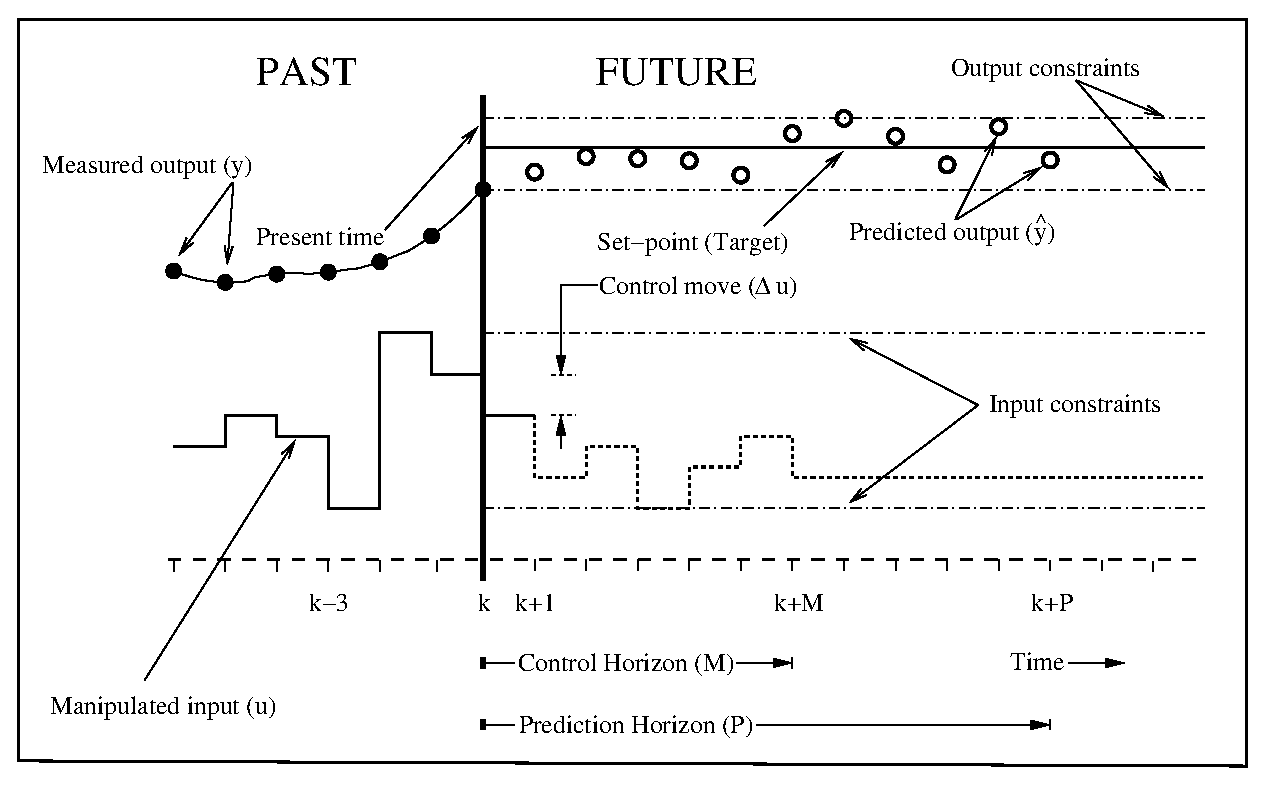
\includegraphics[width=8.2in]{mpc.eps}
\end{center}
\caption{Schematic illustrating receding horizon control.
\label{fig:mpc} }
\end{figure}
\end{quote}
\renewcommand{\baselinestretch}{2}
\small\normalsize
\end{landscape}

This is a my second figure which was placed landscape.  Although I have used the same figure, I have renamed the label to fig:mpc-1.  The second figure now becomes Figure~\ref{fig:mpc-1}.
\begin{landscape}
\renewcommand{\baselinestretch}{1}
\small\normalsize
\begin{quote}
\begin{figure}
\begin{center}
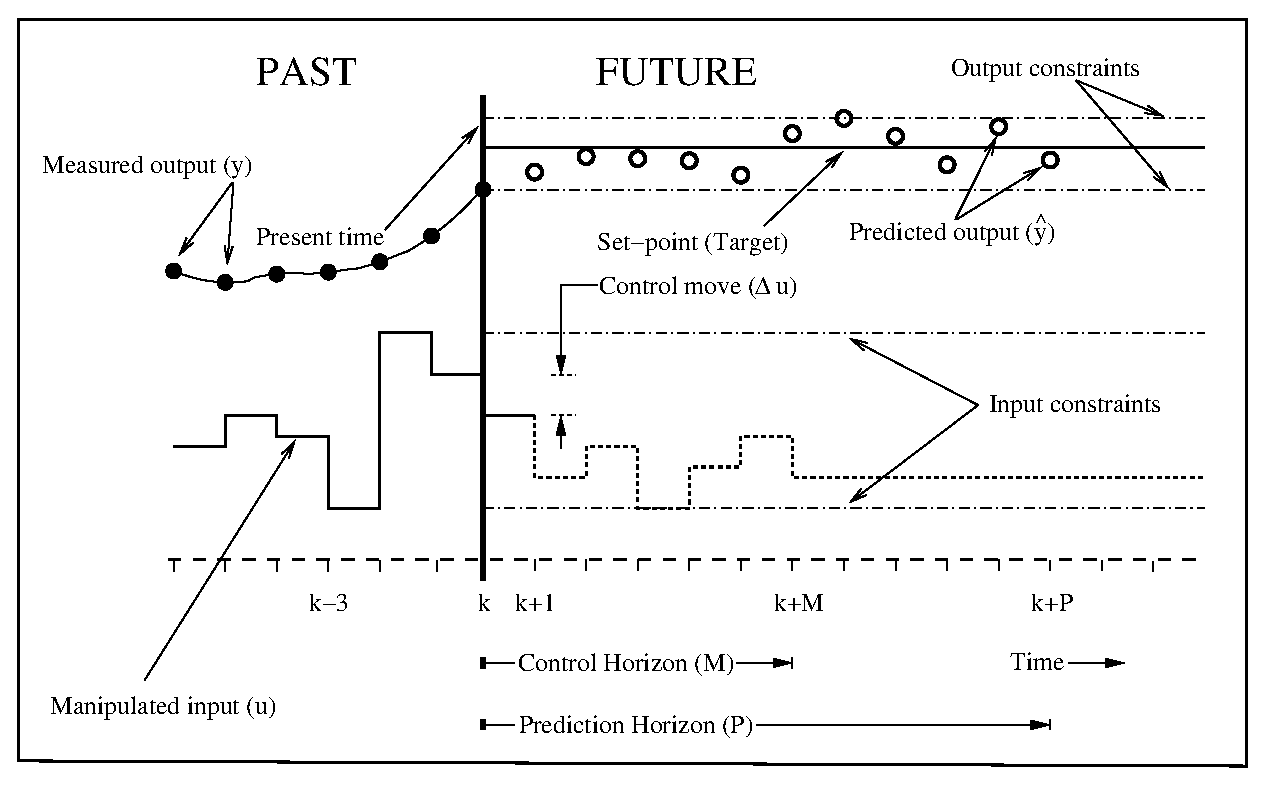
\includegraphics[width=8.2in]{mpc.eps}
\end{center}
\caption[Figure placed landscape on page.]{Schematic illustrating receding horizon control. \label{fig:mpc-1}}
\end{figure}
\end{quote}
\renewcommand{\baselinestretch}{2}
\small\normalsize
\end{landscape}

\subsection{Numbering Figures}

If you wish your figures to be numbered 1-100 without any reference to the chapter (e.g., Figure 1.1, 2.1, etc.), change the first line of your mainthesis.tex file to read \begin{verbatim}"\documentclass[12pt]{thesis-2}".\end{verbatim}  

\subsubsection{This is a Subsubsection}

This is my first subsubsection in Chapter 1.


\section[Short Titles]{Short Titles in the Table of Contents, List of Figures, or List of Tables}

The Table of Contents, List of Figures, or List of Tables usually show the entire title of a section, subsection, etc. or table, or the entire caption of a figure.  If you put a short title in square brackets after \begin{verbatim} \section, \table, or \figure, \end{verbatim} the short title will show in your Table of Contents or lists.

\renewcommand{\baselinestretch}{1}
\small\normalsize

\begin{verbatim}
\section[Short Title]{Title of Section} 
\subsection[Short Title]{Title of Subsection} 
\end{verbatim}

or when using a caption in a figure or table
\begin{verbatim}
\caption[Short Caption]{Full text of the caption.}
\end{verbatim}

\renewcommand{\baselinestretch}{2}
\small\normalsize

\section{Figures on Text Page}

Normally figures in the thesis are placed on a page by themselves.  The following figure is placed on the page with text before and after the figure by adding [!!h] after \begin{verbatim} \begin{figure}[!!h] \end{verbatim}.  Please note that the figure label is placed within the caption.

\renewcommand{\baselinestretch}{1}
\large\normalsize

\begin{verbatim}
\begin{figure}[!!h]
 \begin{center}
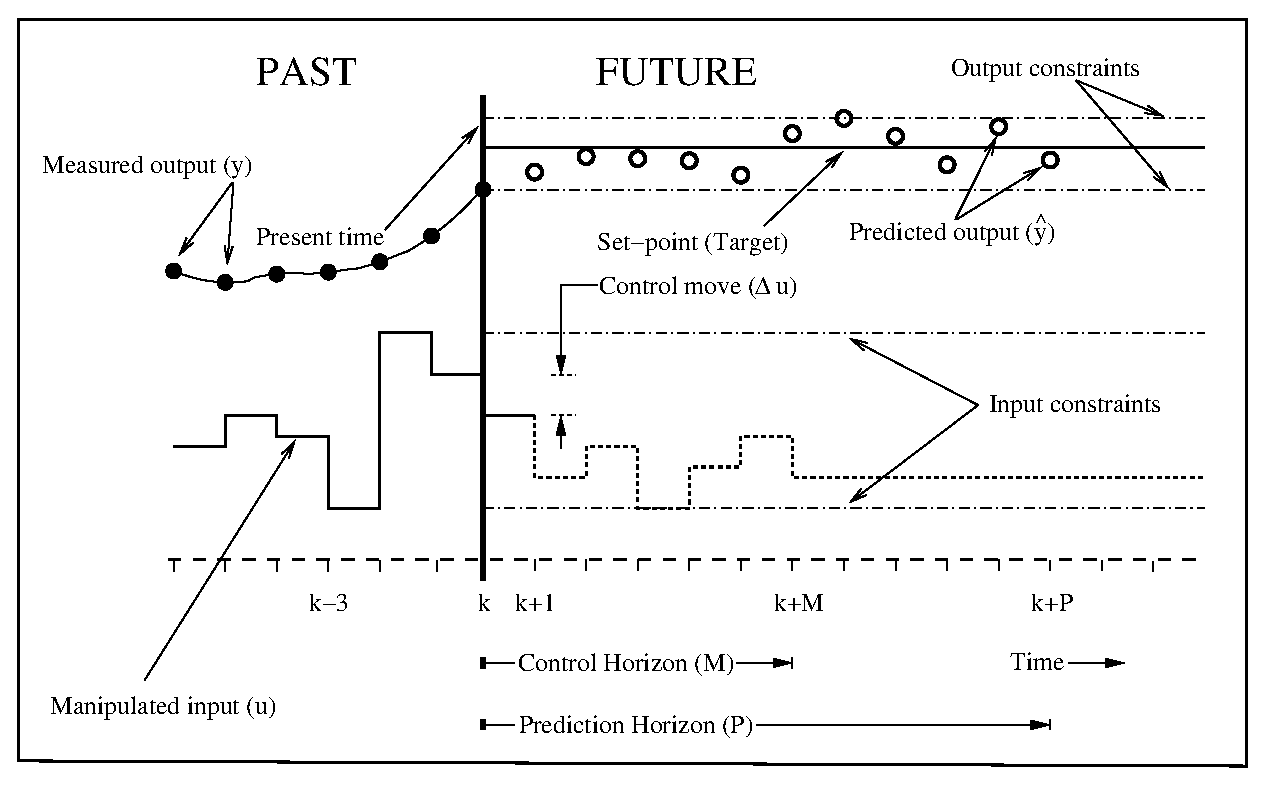
\includegraphics[width=5in]{mpc.eps}
\end{center}
\caption[Short title]{Schematic illustrating receding horizon control.
\label{fig:mpc-2}}
\end{figure}
\end{verbatim}

\begin{figure}[!!h]
 \begin{center}
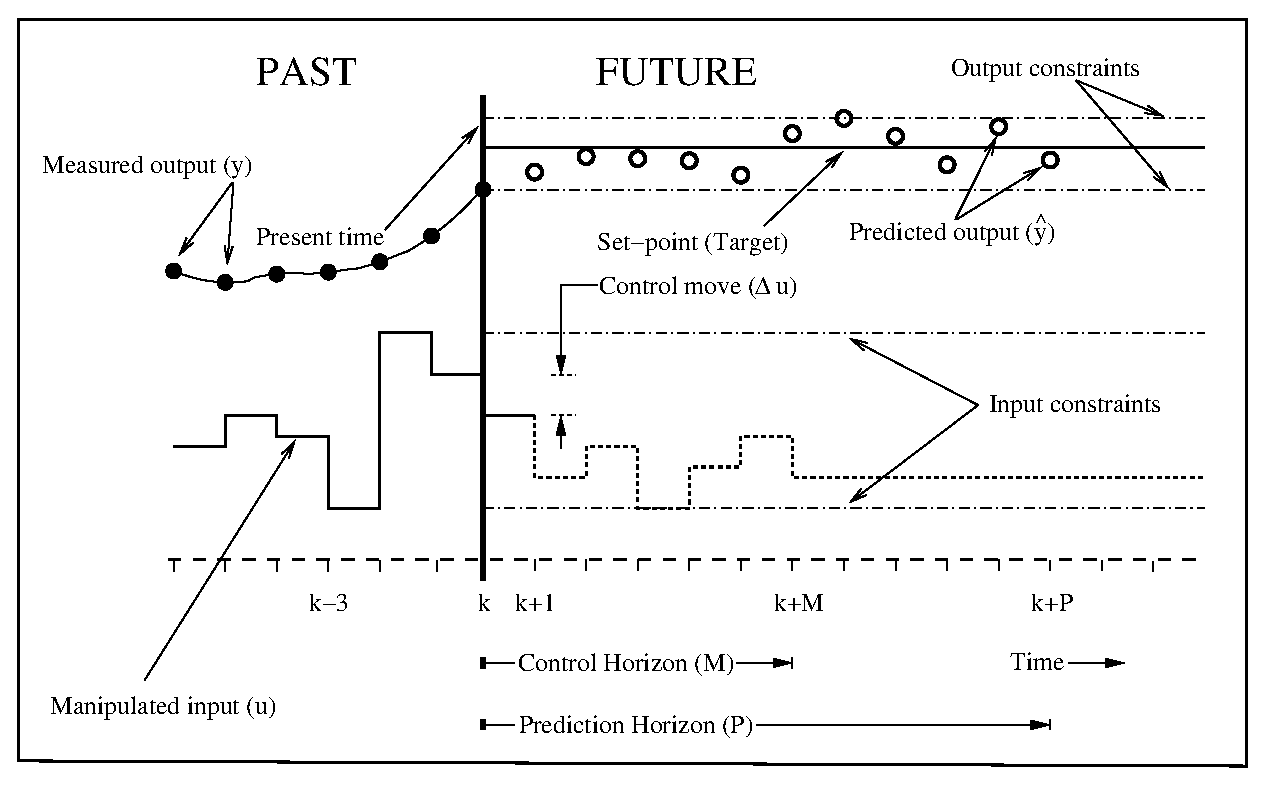
\includegraphics[width=5in]{mpc.eps}
\end{center}
\caption{Schematic illustrating receding horizon control. \label{fig:mpc-2}}
\end{figure}

\renewcommand{\baselinestretch}{2}
\large\normalsize

This does not necessarily mean that the text before and after the figure will be exactly what you want.  Remember Latex will place the figure where it will fit on the page the best.   The previous figure is Figs.~\ref{fig:mpc-2}. 

\section{Wrapping Text around Figure}


\renewcommand{\baselinestretch}{1}
\begin{wrapfigure}{r}{0.4\textwidth}
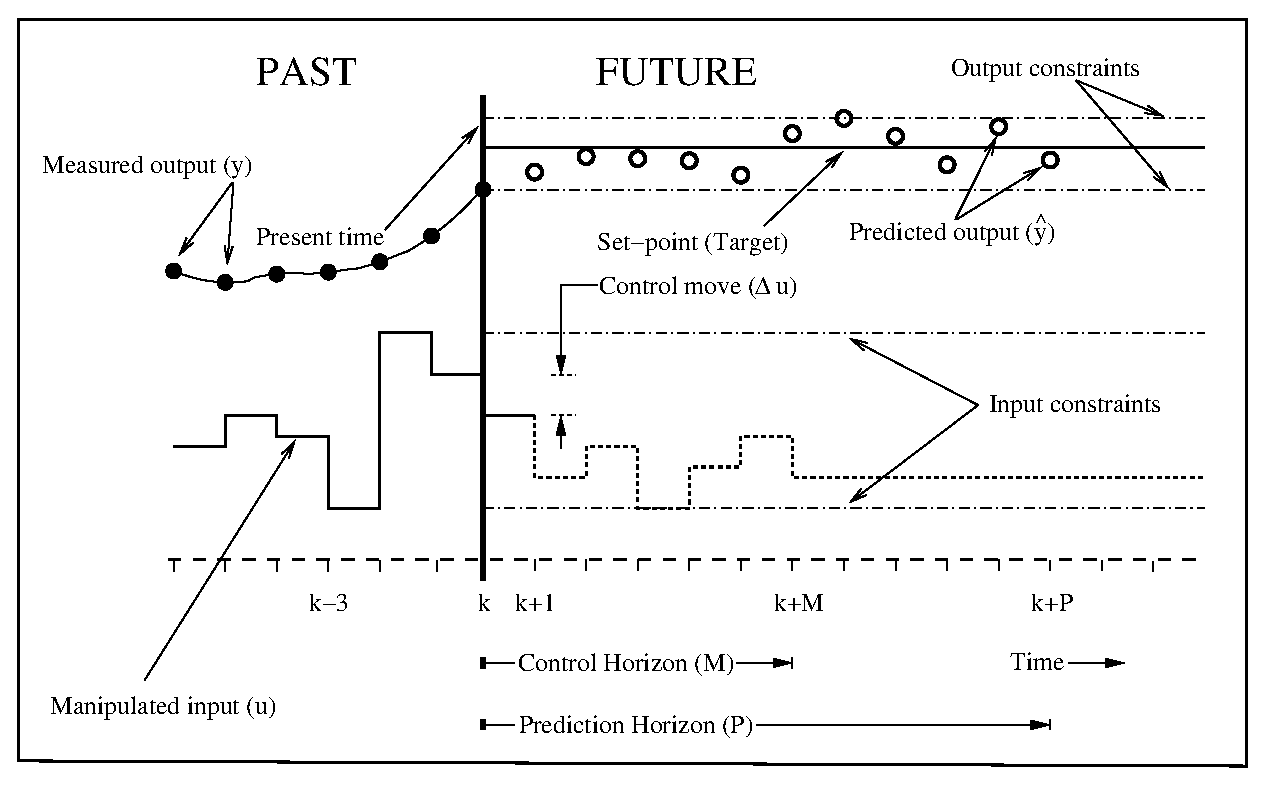
\includegraphics[width=0.4\textwidth]{mpc.eps}
\caption{ Text wrap around figure. \label{fig:test}}
\end{wrapfigure}

\renewcommand{\baselinestretch}{2}
\large\normalsize

By way of summary, at the end of the activity, I reminded the class of what we'd done:  by considering relatively nearby galaxies whose distance we had measured by some other means, we were able to establish a relationship locally between redshift and distance.  
By way of summary, at the end of the activity, I reminded the class of what we'd done:  by considering relatively nearby galaxies whose distance we had measured by some other means, we were able to establish a relationship locally between redshift and distance.  
By way of summary, at the end of the activity, I reminded the class of what we'd done:  by considering relatively nearby galaxies whose distance we had measured by some other means, we were able to establish a relationship locally between redshift and distance.  
By way of summary, at the end of the activity, I reminded the class of what we'd done:  by considering relatively nearby galaxies whose distance we had measured by some other means, we were able to establish a relationship locally between redshift and distance.  See Fig.~\ref{fig:test}.


\section{LaTeX -- A Typesetting Program}

A 13-page explanation of some of the features of LaTeX can be downloaded from http://www.jgsee.kmutt.ac.th/exell/General/LaTeX.html.


\section{Using Bibtex}

Using Bibtex with Latex documents is not difficult.  The bulk of the work is organizing your bibtex file, which is a data base compiled by you of the articles, books, etc. which you use in the bibliographies or reference sections of your publications.  

I have linked several files to this webpage, which will be helpful when you are using Bibtex.  These files can be downloaded from http://www.ireap.umd.edu/ireap/theses/bibtex.  Please read the file "BibtexInstructions.pdf".  The first two pages explain how to set up and run Bibtex; the remaining pages were taken from a published article and show how the references were cited in the .tex file.   The files BibtexInstructions.tex, Galactic.bib, Dottie.bib are the original .tex files used for BibtexInstructions.pdf.  The file BibtexSamples.tex contains examples of the information needed for the various publications you wish to reference (e.g., articles in refereed journals, books, unpublished articles, conference proceedings, etc.).

If you have questions concerning Bibtex, please contact me at 301-405-4955 or dbrosius at umd.edu.


\section{APS Physical Review Style and Notation Guide}

The following style guide may be downloaded from The American Physical Society at http://forms.aps.org/author/styleguide.pdf:  Physical Review Style and Notation Guide, published by The American Physical Society, compiled and edited by Anne Waldron, Peggy Judd, and Valerie Miller, February 1993.  It may be old, but it is very useful.


%\include{Chapter1-subfigures}
%%%
%% This is file `supertabular.sty',
%% generated with the docstrip utility.
%%
%% The original source files were:
%%
%% supertabular.dtx  (with options: `package')
%% Copyright (C) 1989-2004 Johannes Braams. All rights reserved.
%% 
%% This file was generated from file(s) of the supertabular package.
%% -----------------------------------------------------------------
%% 
%% It may be distributed and/or modified under the
%% conditions of the LaTeX Project Public License, either version 1.3
%% of this license or (at your option) any later version.
%% The latest version of this license is in
%%   http://www.latex-project.org/lppl.txt
%% and version 1.3 or later is part of all distributions of LaTeX
%% version 2003/12/01 or later.
%% 
%% This work has the LPPL maintenance status "maintained".
%% 
%% The Current Maintainer of this work is Johannes Braams.
%% 
%% This file may only be distributed together with a copy of the
%% supertabular package. You may however distribute the supertabular package
%% without such generated files.
%% 
%% The list of all files belonging to the supertabular package is
%% given in the file `manifest.txt.
%% 
%% The list of derived (unpacked) files belonging to the distribution
%% and covered by LPPL is defined by the unpacking scripts (with
%% extension .ins) which are part of the distribution.
%% Sourcefile `supertabular.dtx'.
%%
%% Copyright (C) 1988 by Theo Jurriens
%% Copyright (C) 1990-2004 by Johannes Braams texniek at braams.cistron.nl
%%                            Kersengaarde 33
%%                            2723 BP Zoetermeer NL
%%                       all rights reserved.
%%
%%
\NeedsTeXFormat{LaTeX2e}
\ProvidesPackage{supertabular}
              [2004/02/20 v4.1e the supertabular environment]
\newcount\c@tracingst
\DeclareOption{errorshow}{\c@tracingst\z@}
\DeclareOption{pageshow}{\c@tracingst\tw@}
\DeclareOption{debugshow}{\c@tracingst5\relax}
\ProcessOptions
\newif\if@topcaption \@topcaptiontrue
\def\topcaption{\@topcaptiontrue\tablecaption}
\def\bottomcaption{\@topcaptionfalse\tablecaption}
\long\def\tablecaption{%
  \refstepcounter{table}\@dblarg{\@xtablecaption}}
\long\def\@xtablecaption[#1]#2{%
  \long\gdef\@process@tablecaption{\ST@caption{table}[#1]{#2}}}
\global\let\@process@tablecaption\relax
\newif\ifST@star
\newif\ifST@mp
\newdimen\ST@wd
\newskip\ST@rightskip
\newskip\ST@leftskip
\newskip\ST@parfillskip
\long\def\ST@caption#1[#2]#3{\par%
  \addcontentsline{\csname ext@#1\endcsname}{#1}%
                  {\protect\numberline{%
                      \csname the#1\endcsname}{\ignorespaces #2}}
  \begingroup
    \@parboxrestore
    \normalsize
    \if@topcaption \vskip -10\p@ \fi
    \@makecaption{\csname fnum@#1\endcsname}{\ignorespaces #3}\par
    \if@topcaption \vskip 10\p@ \fi
  \endgroup}
\newcommand\tablehead[1]{%
  \gdef\@tablehead{%
  \noalign{%
      \global\let\@savcr=\\
      \global\let\\=\org@tabularcr}%
    #1%
    \noalign{\global\let\\=\@savcr}}}
\tablehead{}
\newcommand\tablefirsthead[1]{\gdef\@table@first@head{#1}}
\newcommand\tabletail[1]{%
  \gdef\@tabletail{%
    \noalign{%
      \global\let\@savcr=\\
      \global\let\\=\org@tabularcr}%
    #1%
    \noalign{\global\let\\=\@savcr}}}
\tabletail{}
\newcommand\tablelasttail[1]{\gdef\@table@last@tail{#1}}
\newcommand\sttraceon{\c@tracingst5\relax}
\newcommand\sttraceoff{\c@tracingst\z@}
\newcommand\ST@trace[2]{%
  \ifnum\c@tracingst>#1\relax
    \GenericWarning
      {(supertabular)\@spaces\@spaces}
      {Package supertabular: #2}%
  \fi
  }
\newdimen\ST@pageleft
\newcommand*\shrinkheight[1]{%
  \noalign{\global\advance\ST@pageleft-#1\relax}}
\newcommand*\setSTheight[1]{%
  \noalign{\global\ST@pageleft=#1\relax}}
\newdimen\ST@headht
\newdimen\ST@tailht
\newdimen\ST@pagesofar
\newdimen\ST@pboxht
\newdimen\ST@lineht
\newdimen\ST@stretchht
\newdimen\ST@prevht
\newdimen\ST@toadd
\newdimen\ST@dimen
\newbox\ST@pbox
\def\ST@tabularcr{%
  {\ifnum0=`}\fi
  \@ifstar{\ST@xtabularcr}{\ST@xtabularcr}}
\def\ST@xtabularcr{%
  \@ifnextchar[%]
    {\ST@argtabularcr}%
    {\ifnum0=`{\fi}\cr\ST@cr}}
\def\ST@argtabularcr[#1]{%
  \ifnum0=`{\fi}%
  \ifdim #1>\z@
    \unskip\ST@xargarraycr{#1}
  \else
    \ST@yargarraycr{#1}%
  \fi}
\def\ST@xargarraycr#1{%
  \@tempdima #1\advance\@tempdima \dp \@arstrutbox
  \vrule \@height\z@ \@depth\@tempdima \@width\z@ \cr
  \noalign{\global\ST@toadd=#1}\ST@cr}
\def\ST@yargarraycr#1{%
  \cr\noalign{\vskip #1\global\ST@toadd=#1}\ST@cr}
\def\ST@startpbox#1{%
  \setbox\ST@pbox\vtop\bgroup\hsize#1\@arrayparboxrestore}
\def\ST@astartpbox#1{%
  \bgroup\hsize#1%
  \setbox\ST@pbox\vtop\bgroup\hsize#1\@arrayparboxrestore}
\def\ST@endpbox{%
  \@finalstrut\@arstrutbox\par\egroup
  \ST@dimen=\ht\ST@pbox
  \advance\ST@dimen by \dp\ST@pbox
  \ifnum\ST@pboxht<\ST@dimen
    \global\ST@pboxht=\ST@dimen
  \fi
  \ST@dimen=\z@
  \box\ST@pbox\hfil}
\def\ST@aendpbox{%
  \@finalstrut\@arstrutbox\par\egroup
  \ST@dimen=\ht\ST@pbox
  \advance\ST@dimen by \dp\ST@pbox
  \ifnum\ST@pboxht<\ST@dimen
    \global\ST@pboxht=\ST@dimen
  \fi
  \ST@dimen=\z@
  \unvbox\ST@pbox\egroup\hfil}
\def\estimate@lineht{%
  \ST@lineht=\arraystretch \baslineskp
  \global\advance\ST@lineht by 1\p@
  \ST@stretchht\ST@lineht\advance\ST@stretchht-\baslineskp
  \ifdim\ST@stretchht<\z@\ST@stretchht\z@\fi
  \ST@trace\tw@{Average line height: \the\ST@lineht}%
  \ST@trace\tw@{Stretched line height: \the\ST@stretchht}%
  }
\def\@calfirstpageht{%
  \ST@trace\tw@{Calculating height of tabular on first page}%
  \global\ST@pagesofar\pagetotal
  \global\ST@pageleft\@colroom
  \ST@trace\tw@{Height of text = \the\pagetotal; \MessageBreak
                Height of page = \the\ST@pageleft}%
  \if@twocolumn
    \ST@trace\tw@{two column mode}%
    \if@firstcolumn
     \ST@trace\tw@{First column}%
      \ifnum\ST@pagesofar > \ST@pageleft
        \global\ST@pageleft=2\ST@pageleft
        \ifnum\ST@pagesofar > \ST@pageleft
          \newpage\@calnextpageht
          \ST@trace\tw@{starting new page}%
        \else
          \ST@trace\tw@{Second column}%
          \global\advance\ST@pageleft -\ST@pagesofar
          \global\advance\ST@pageleft -\@colroom
        \fi
      \else
        \global\advance\ST@pageleft by -\ST@pagesofar
        \global\ST@pagesofar\z@
      \fi
    \else
      \ST@trace\tw@{Second column}
      \ifnum\ST@pagesofar > \ST@pageleft
        \ST@trace\tw@{starting new page}%
        \newpage\@calnextpageht
      \else
        \global\advance\ST@pageleft by -\ST@pagesofar
        \global\ST@pagesofar\z@
      \fi
    \fi
  \else
    \ST@trace\tw@{one column mode}%
    \ifnum\ST@pagesofar > \ST@pageleft
      \ST@trace\tw@{starting new page}%
      \newpage\@calnextpageht
    \else
      \global\advance\ST@pageleft by -\ST@pagesofar
      \global\ST@pagesofar\z@
    \fi
  \fi
  \ST@trace\tw@{Available height: \the\ST@pageleft}%
  \ifx\@@tablehead\@empty
    \ST@headht=\z@
  \else
    \setbox\@tempboxa=\vbox{\@arrayparboxrestore
      \ST@restore
      \expandafter\tabular\expandafter{\ST@tableformat}%
      \@@tablehead\endtabular}%
    \ST@headht=\ht\@tempboxa\advance\ST@headht\dp\@tempboxa
  \fi
  \ST@trace\tw@{Height of head: \the\ST@headht}%
  \ifx\@tabletail\@empty
    \ST@tailht=\z@
  \else
    \setbox\@tempboxa=\vbox{\@arrayparboxrestore
      \ST@restore
      \expandafter\tabular\expandafter{\ST@tableformat}
        \@tabletail\endtabular}
    \ST@tailht=\ht\@tempboxa\advance\ST@tailht\dp\@tempboxa
  \fi
  \advance\ST@tailht by \ST@lineht
  \ST@trace\tw@{Height of tail: \the\ST@tailht}%
  \ST@trace\tw@{Maximum height of tabular: \the\ST@pageleft}%
  \@tempdima\ST@headht
  \advance\@tempdima\ST@lineht
  \advance\@tempdima\ST@tailht
  \ST@trace\tw@{Minimum height of tabular: \the\@tempdima}%
  \ifnum\@tempdima>\ST@pageleft
    \ST@trace\tw@{starting new page}%
    \newpage\@calnextpageht
  \fi
}
\def\@calnextpageht{%
  \ST@trace\tw@{Calculating height of tabular on next page}%
  \global\ST@pageleft\@colroom
  \global\ST@pagesofar=\z@
  \ST@trace\tw@{Maximum height of tabular: \the\ST@pageleft}%
  }
\def\x@supertabular{%
  \let\org@tabular\tabular
  \let\tabular\inner@tabular
  \expandafter\let
    \csname org@tabular*\expandafter\endcsname
    \csname tabular*\endcsname
  \expandafter\let\csname tabular*\expandafter\endcsname
    \csname inner@tabular*\endcsname
  \if@topcaption \@process@tablecaption \fi
  \global\let\@oldcr=\\
  \def\baslineskp{\baselineskip}%
  \ifx\undefined\@classix
    \let\org@tabularcr\@tabularcr
    \let\@tabularcr\ST@tabularcr
    \let\org@startpbox=\@startpbox
    \let\org@endpbox=\@endpbox
    \let\@@startpbox=\ST@startpbox
    \let\@@endpbox=\ST@endpbox
  \else
    \let\org@tabularcr\@arraycr
    \let\@arraycr\ST@tabularcr
    \let\org@startpbox=\@startpbox
    \let\org@endpbox=\@endpbox
    \let\@startpbox=\ST@astartpbox
    \let\@endpbox=\ST@aendpbox
  \fi
  \ifx\@table@first@head\undefined
    \let\@@tablehead=\@tablehead
  \else
    \let\@@tablehead=\@table@first@head
  \fi
  \let\ST@skippage\ST@skipfirstpart
  \estimate@lineht
  \@calfirstpageht
  \noindent
  }
\def\supertabular{%
  \@ifnextchar[{\@supertabular}%]
               {\@supertabular[]}}
\def\@supertabular[#1]#2{%
  \def\ST@tableformat{#2}%
  \ST@trace\tw@{Starting a new supertabular}%
  \global\ST@starfalse
  \global\ST@mpfalse
  \x@supertabular
  \expandafter\org@tabular\expandafter{\ST@tableformat}%
  \@@tablehead}
\@namedef{supertabular*}#1{%
  \@ifnextchar[{\@nameuse{@supertabular*}{#1}}%
               {\@nameuse{@supertabular*}{#1}[]}%]
  }
\@namedef{@supertabular*}#1[#2]#3{%
  \ST@trace\tw@{Starting a new supertabular*}%
  \def\ST@tableformat{#3}%
  \ST@wd=#1\relax
  \global\ST@startrue
  \global\ST@mpfalse
  \x@supertabular
  \expandafter\csname org@tabular*\expandafter\endcsname
  \expandafter{\expandafter\ST@wd\expandafter}%
  \expandafter{\ST@tableformat}%
  \@@tablehead}%
\def\mpsupertabular{%
  \@ifnextchar[{\@mpsupertabular}%]
               {\@mpsupertabular[]}}
\def\@mpsupertabular[#1]#2{%
  \def\ST@tableformat{#2}%
  \ST@trace\tw@{Starting a new mpsupertabular}%
  \global\ST@starfalse
  \global\ST@mptrue
  \ST@rightskip \rightskip
  \ST@leftskip \leftskip
  \ST@parfillskip \parfillskip
  \x@supertabular
  \minipage{\columnwidth}%
  \parfillskip\ST@parfillskip
  \rightskip \ST@rightskip
  \leftskip \ST@leftskip
  \noindent\expandafter\org@tabular\expandafter{\ST@tableformat}%
  \@@tablehead}
\@namedef{mpsupertabular*}#1{%
  \@ifnextchar[{\@nameuse{@mpsupertabular*}{#1}}%
               {\@nameuse{@mpsupertabular*}{#1}[]}%]
  }
\@namedef{@mpsupertabular*}#1[#2]#3{%
  \ST@trace\tw@{Starting a new mpsupertabular*}%
  \def\ST@tableformat{#3}%
  \ST@wd=#1\relax
  \global\ST@startrue
  \global\ST@mptrue
  \ST@rightskip \rightskip
  \ST@leftskip \leftskip
  \ST@parfillskip \parfillskip
  \x@supertabular
  \minipage{\columnwidth}%
  \parfillskip\ST@parfillskip
  \rightskip \ST@rightskip
  \leftskip \ST@leftskip
  \noindent\expandafter\csname org@tabular*\expandafter\endcsname
  \expandafter{\expandafter\ST@wd\expandafter}%
  \expandafter{\ST@tableformat}%
  \@@tablehead}%
\def\endsupertabular{%
  \ifx\@table@last@tail\undefined
    \@tabletail
  \else
    \@table@last@tail
  \fi
  \csname endtabular\ifST@star*\fi\endcsname
  \ST@restore
  \if@topcaption
  \else
    \@process@tablecaption
    \@topcaptiontrue
  \fi
  \global\let\\\@oldcr
  \global\let\@process@tablecaption\relax
  \ST@trace\tw@{Ended a supertabular\ifST@star*\fi}%
  }
\expandafter\let\csname endsupertabular*\endcsname\endsupertabular
\def\endmpsupertabular{%
  \ifx\@table@last@tail\undefined
    \@tabletail
  \else
    \@table@last@tail
  \fi
  \csname endtabular\ifST@star*\fi\endcsname
  \endminipage
  \ST@restore
  \if@topcaption
  \else
    \@process@tablecaption
    \@topcaptiontrue
  \fi
  \global\let\\\@oldcr
  \global\let\@process@tablecaption\relax
  \ST@trace\tw@{Ended a mpsupertabular\ifST@star*\fi}%
  }
\expandafter\let\csname endmpsupertabular*\endcsname\endmpsupertabular
\def\ST@restore{%
  \ifx\undefined\@classix
    \let\@tabularcr\org@tabularcr
  \else
    \let\@arraycr\org@tabularcr
  \fi
  \let\@startpbox\org@startpbox
  \let\@endpbox\org@endpbox
  }
\def\inner@tabular{%
  \ST@restore
  \let\\\@oldcr
  \noindent
  \org@tabular}
\@namedef{inner@tabular*}{%
  \ST@restore
  \let\\\@oldcr
  \noindent
  \csname org@tabular*\endcsname}
\def\ST@cr{%
  \noalign{%
    \ifnum\ST@pboxht<\ST@lineht
      \global\advance\ST@pageleft -\ST@lineht
      \global\ST@prevht\ST@lineht
    \else
     \ST@trace\thr@@{Added par box with height \the\ST@pboxht}%
      \global\advance\ST@pageleft -\ST@pboxht
      \global\advance\ST@pageleft -0.1\ST@pboxht
      \global\advance\ST@pageleft -\ST@stretchht
      \global\ST@prevht\ST@pboxht
      \global\ST@pboxht\z@
    \fi
    \global\advance\ST@pageleft -\ST@toadd
    \global\ST@toadd=\z@
    \ST@trace\thr@@{Space left for tabular: \the\ST@pageleft}%
  }
  \noalign{\global\let\ST@next\@empty}%
  \ifnum\ST@pageleft<\z@
    \ST@skippage
  \else
    \noalign{\global\@tempdima\ST@tailht
      \global\advance\@tempdima\ST@prevht
    \ifST@mp
      \ifvoid\@mpfootins\else
        \global\advance\@tempdima\ht\@mpfootins
        \global\advance\@tempdima 3pt
      \fi
    \fi}
    \ifnum\ST@pageleft<\@tempdima
      \ST@newpage
    \fi
  \fi
  \ST@next}
\def\ST@skipfirstpart{%
  \noalign{%
    \ST@trace\tw@{Tabular too high, moving to next page}%
    \global\advance\ST@pageleft\pagetotal
    \global\ST@pagesofar\z@
    \newpage
    \global\let\ST@skippage\ST@newpage
    }}
\def\ST@newpage{%
  \noalign{\ST@trace\tw@{Starting new page, writing tail}}%
  \@tabletail
  \ifST@star
    \csname endtabular*\endcsname
  \else
    \endtabular
  \fi
  \ifST@mp
    \endminipage
  \fi
  \global\let\ST@skippage\ST@newpage
  \newpage\@calnextpageht
  \let\ST@next\@tablehead
  \ST@trace\tw@{writing head}%
  \ifST@mp
    \noindent\minipage{\columnwidth}%
    \parfillskip\ST@parfillskip
    \rightskip \ST@rightskip
    \leftskip \ST@leftskip
  \fi
  \noindent
  \ifST@star
    \expandafter\csname org@tabular*\expandafter\endcsname
    \expandafter{\expandafter\ST@wd\expandafter}%
    \expandafter{\ST@tableformat}%
  \else
    \expandafter\org@tabular\expandafter{\ST@tableformat}%
  \fi}
\endinput
%%
%% End of file `supertabular.sty'.

%Appendix
\appendix
\renewcommand{\thechapter}{A}

\chapter{Overview}

Here is an overview of the contents of Appendix A.

\section{Details}

Appendices contain details.  Don't forget the picture.


%Figure A.1
\begin{figure}
\begin{center}
\includegraphics[0in,0in][3.25in,4.266in]{nlsetime.eps}
\end{center}
\renewcommand{\baselinestretch}{1}
\small\normalsize
\begin{quote}
\caption{Multimode pulse input to the NLSE: (a) input pulse in time
domain and (b) input spectrum.}
\label{figA.1}
\end{quote}
\end{figure}
\renewcommand{\baselinestretch}{2}
\small\normalsize



\renewcommand{\baselinestretch}{1}
\small\normalsize
\begin{thebibliography}{99}
\setlength{\parskip}{1em}

\bibitem{Agrawal1} G.P. Agrawal, {\em Nonlinear Fiber Optics} (Academic
Press, San Diego, CA, 2001), Chap. 1.
\bibitem{Bloembergen} N. Bloembergen, {\em Nonlinear Optics} (Benjamin,
Reading, MA, 1977).
\bibitem{Shen} Y.R. Shen, {\em Principles of Nonlinear Optics} (Wiley, New
York, 1984).
\bibitem{Butcher} P.N. Butcher and D.N. Cotter, {\em The Elements of
Nonlinear Optics} (Cambridge University Press, Cambridge, UK, 1990).
\bibitem{Boyd} R.W. Boyd, {\em Nonlinear Optics} (Academic Press, San Diego,
CA, 1992).
\bibitem{Newell} A.C. Newell and J.V. Moloney {\em Nonlinear Optics (Advanced Topics in the Interdisciplinary Mathematical Sciences)} (Westview Press, Boulder, CO, April 1992). 
\bibitem{Marcuse} D. Marcuse,{\em Light Transmission Optics} (Van Nostrand
Reinhold, New York, 1982), Chaps. 8 and 12.
\bibitem{Agrawal2} G.P. Agrawal, {\em Nonlinear Fiber Optics} (Academic
Press, San Diego, CA, 2001), Chap. 2.
\bibitem{Diament} P. Diament, {\em Wave Transmission and Fiber Optics}
(Macmillan, New York, 1990).
\bibitem{Zakharov} V.E. Zakharov and A.Shabat, Sov. Phys. JETP 
\textbf{34}, 62 (1972)
\bibitem{Hardin} R.H. Hardin and F.D. Tappert, SIAM
Rev. Chronicle \textbf{15}, 423 (1973).
\bibitem{Fisher} R.A.Fisher and
W.K. Bischel, Appl. Phys. Lett. \textbf{23}, 661 (1973); J. Appl. Phys
\textbf{46}, 4921 (1975).
\bibitem{Cooley} J.W. Cooley and J.W. Tukey,
Math. Comput. \textbf{19}, 297 (1965).
\bibitem{Trebino} R. Trebino, D.J. Kane, "Using phase retrieval to measure
the intensity and phase of ultrashort pulses: frequency resolved optical gating," J. Opt. Soc. Am. B \textbf{10}, 1101 (1993). 
\bibitem{Kanejqe} D.J. Kane, R. Trebino, "Characterization of Arbitrary Femtosecond Pulses Using Frequency-Resolved Optical Gating," IEEE J. Quant. Elect. \textbf{29}, 571 (1993). 
\bibitem{Kaneoptlett} D.J. Kane, R. Trebino, "Single-shot measurement of the intensity and phase of an arbitrary ultrashort pulse  by using frequency-resolved optical gating," Opt. Lett. \textbf{10}, 1101 (1993).
\bibitem{OShealett}P. O'Shea, M. Kimmel, X. Gu, R. Trebino, "Highly simplified device for ultrashort-pulse measurement," Opt. Lett. \textbf{26}, 932 (2001).
\bibitem{Agrawal3} G.P. Agrawal, {\em Nonlinear Fiber Optics} (Academic
Press, San Diego, CA, 2001), Chap. 3.
\bibitem{Agrawal4} G.P. Agrawal, {\em Nonlinear Fiber Optics} (Academic
Press, San Diego, CA, 2001), Chap. 4.
\bibitem{Agrawal10} G.P. Agrawal, {\em Nonlinear Fiber Optics} (Academic
Press, San Diego, CA, 2001), Chap. 10.
\bibitem{Agrawal7} G.P. Agrawal, {\em Nonlinear Fiber Optics} (Academic
Press, San Diego, CA, 2001), Chap. 7.
\bibitem{Agrawal6} G.P. Agrawal, {\em Nonlinear Fiber Optics} (Academic
Press, San Diego, CA, 2001), Chap. 6.
\bibitem{Stolen} R.H. Stolen, E.P. Ippen, and A.R. Tynes,
Appl. Phys. Lett. \textbf{20}, 62 (1972). 
\bibitem{Ippen} E.P. Ippen and R.H. Stolen, Appl. Phys. Lett. \textbf{21}, 
539 (1972). 
\bibitem{Smith} R.G. Smith, Appl. Opt. \textbf{11}, 2489 (1972).
\bibitem{Agrawal9} G.P. Agrawal, {\em Nonlinear Fiber Optics} (Academic
Press, San Diego, CA, 2001), Chap. 9.
\bibitem{Agrawal8} G.P. Agrawal, {\em Nonlinear Fiber Optics} (Academic
Press, San Diego, CA, 2001), Chap. 8.
\bibitem{hart1} D.L. Hart, Arthur F. Judy, Rajarshi Roy and James W. Beletic, Phys. Rev. E \textbf{57}, 4757 (1998); D.L. Hart, Arthur F. Judy, T.A.B. Kennedy, Rajarshi Roy and K. Stoev, Phys. Rev. A \textbf{50}, 1807 (1994).   
\bibitem{ito} K. Ito, {\em Lectures on Stochastic Processes} (Tata Institute of Fundamental Research, Bombay, 1960).
\bibitem{stratanovich} R.L. Stratanovich, {\em Topics in the Theory of Random Noise}, Vols I. and II. (Gordon \& Breach, New York, 1963).
\bibitem{risken} H. Risken, {\em The Fokker-Planck Equation} (Springer-Verlag, Berlin, 1989).
\bibitem{werner2} M.J. Werner and P.D. Drummond, J. Comput. Phys. \textbf{132}, 312 (1997).
\bibitem{drummond1} P.D. Drummond and I.K. Mortimer, J. Comput. Phys. \textbf{93}, 144 (1991).
\bibitem{carter3} S.J. Carter, Phys. Rev. A. \textbf{51}, 3274 (1995).
\bibitem{thompson1} J.R. Thompson and Rajarshi Roy, Phys. Rev. A \textbf{43}, 4987 (1991).
\bibitem{boxmuller} W.H. Press, S.A. Teukolsky, W.T. Vetterling and B.P. Flannery, {\em Numerical Recipes in Fortran: The Art of Scientific Computing} (Cambridge University Press, Cambridge, 1992).
\bibitem{headley} C. Headley, G.P. Agrawal, IEEE J. Quantum Electron. \textbf{QE-31}, 2058 (1995), C. Headley, G.P. Agrawal J. Opt. Soc. Am. B. \textbf{13}, 2170 (1995).
\bibitem{perlmutter1} S.H. Perlmutter, M.D. Levenson, R.M. Shelby and
M.B. Weisman, Phys. Rev. Lett. \textbf{61} 1388, 1988.
\bibitem{abdullaev} F. Kh. Abdullaev, J.H. Hensen, S. Bischoff and M.P. Sorensen, J. Opt. Soc. Am. B. \textbf{15}, 2424 (1998); F. Kh. Abdullaev, J.G. Caputo, and Nikos Flytzanis, Phys. Rev E. \textbf{50}, 1552 (1994).
\bibitem{glenn} William H. Glenn, IEEE J. Quantum Electron. \textbf{QE-25}, 1218 (1989).
\bibitem{Trebinobook} R. Trebino. {\em Frequency-Resolved Optical Gating: The Measurement of Ultrashort Laser Pulses} (Kluwer Academic 2002).
\bibitem{Agrawal} G.P. Agrawal {\em Nonlinear Fiber Optics} (Academic,
San Diego, 2001).
\bibitem{Dudley} J.M. Dudley, X. Gu, L. Xu, M. Kimmel, E. Zeek, P. O'Shea, R. Trebino, S. Coen, R.S. Windeler, "Cross-correlation frequency resolved optical gating analysis of broadband continuum generation in photonic crystal fiber: simulations and experiments," Opt. Express \textbf{10}, 1215 (2002).
\bibitem{Liu1} Q.D. Liu, J.T. Chen, Q.Z. Wang, P.P. Ho, and R.R. Alfano, "Single pulse degenerate-cross-phase modulation in a single-mode optical fiber," Opt. Lett. \textbf{20}, 542 (1995).
\bibitem{Sylvestre} T. Sylvestre, H. Maillotte, E. Lantz, and D. Gindre "Combined spectral effects of pulse walk-off and degenerate cross-phase modulation in birefringent fibers", Journal of Nonlinear Optical Physics and Materials 6, 313-320 (1997).
\bibitem{Liu2} Q.D. Liu, L. Shi, P.P. Ho, R.R. Alfano, R.J. Essiambre, and G.P. Agrawal, "Degenerate cross-phase modulation of femtosecond laser pulses in a birefringent single-mode fiber," IEEE Photon. Tech. Lett. \textbf{9}, 1107 (1997). 
\bibitem{Omenetto1} F.G. Omenetto, B.P. Luce, D. Yarotski and A.J. Taylor, "Observation of chirped soliton dynamics at l= 1.55 mm in a single-mode optical fiber with frequency-resolved optical gating," Opt. Lett. \textbf{24}, 1392 (1999).
% 1.55 micron regime - check for more recent papers by Omenetto use both web-sci and inspec
\bibitem{Omenetto2} F.G. Omenetto, Y. Chung, D. Yarotski, T. Shaefer, I. Gabitov and A.J. Taylor, "Phase analysis of nonlinear femtosecond pulse propagation and self-frequency shift in optical fibers," Opt. Commun. \textbf{208}, 191 (2002). 
\bibitem{Omenetto3} F.G. Omenetto, J.W. Nicholson, B.P. Luce, D. Yarotski, A.J. Taylor, "Shaping, propagation and characterization of ultrafast pulses in optical fibers," Appl. Phys. B \textbf{70}[Suppl.], S143 (2000).
\bibitem{Nishizawa1} N. Nishizawa and T. Goto, "Experimental analysis of ultrashort pulse propagation in optical fibers around zero-dispersion region using cross-correlation frequency resolved optical gating," Opt. Express \textbf{8}, 328 (2001).
\bibitem{Nishizawa2} N. Nishizawa and T. Goto, "Trapped pulse generation by femtosecond soliton pulse in birefringent optical fibers," Opt. Express \textbf{10}, 256 (2002).
\bibitem{Nishizawa3} N. Nishizawa and T. Goto, "Characteristics of pulse trapping by use of ultrashort soliton pulses in optical fibers across the zero-dispersion wavelength," Opt. Express \textbf{10}, 1151 (2002).
\bibitem{Nishizawa4} N. Nishizawa and T. Goto, "Ultrafast all optical switching by use of pulse trapping across zero-dispersion wavelength," Opt. Express \textbf{11}, 359 (2003).
% All of Nishizawa and Goto papers are related to 1.3 micron experiments and simulations.
\bibitem{Ogawa}, K. Ogawa, M.D. Pelusi, "Characterization of ultrashort optical pulses in a dispersion-managed fiber link using two-photon absorption frequency-resolved optical gating," Opt. Commun. \textbf{198}, 83-87 (2001).
\bibitem{Altes} R.A. Altes, "Detection, estimation, and classification
with spectrograms," J. Acoust. Soc. Am. \textbf{67}(4), 1232 (1980).
\bibitem{Christian} A. Christian Silva, "GRENOUILLE - Practical Issues," unpublished.
\bibitem{Mejia} J. Garduno-Mejia, A.H. Greenaway, and D.T. Reid, "Designer
femtosecond pulses using adaptive optics," Opt. Express \textbf{11}
2030 (2003).
\bibitem{OSheaexpress1} P. O'Shea, M. Kimmel, X. Gu, R. Trebino, "Increased-bandwidth in ultrashort-pulse measurement using an angle-dithered nonlinear-optical crystal," Opt. Express \textbf{7}, 342 (2000).
\bibitem{OSheaexpress2} P. O'Shea, M. Kimmel, R. Trebino, "Increased phase-matching bandwidth in simple ultrashort-laser-pulse measurements," J. Opt. B \textbf{4}, 44 (2002).
\bibitem{Akturk} S. Akturk, M. Kimmel, P. O'Shea, R. Trebino, "Measuring pulse-front tilt in ultrashort pulses using GRENOUILLE", Opt. Express \textbf{11}, 491 (2003).
\bibitem{Blow} K. J. Blow, D. Wood, "Theoretical Description of Transient Stimulated Raman Scattering in Optical Fibers," IEEE J. Quant. Elect. \textbf{25}, 2665 (1989).
\bibitem{Stolen2} R.H. Stolen, J.P. Gordon, W.J. Tomlinson,
J. Opt. Soc. Am. B \textbf{6}, 1159 (1989).
\bibitem{Mamyshev} P.V. Mamyshev and S.V. Chernikov, Sov. Lightwave
Commun. \textbf{2}, 97 (1992).
\bibitem{Headleythesis} C. Headley III, \em{Ultrafast Stimulated Raman
Scattering in Optical Fibers}, Ph.D. Thesis, University of Rochester,
NY (1995).
\end{thebibliography}

%When using Bibtex, delete the previous line and use the following
%three lines.  
%\newpage
%\bibliographystyle{unsrt} 
%\bibliography{Galactic,Dottie} %replace "Galactic,Dottie" with the
%                 file name(s) of your bib file(s)

\end{document}
